% Created by tikzDevice version 0.11 on 2018-05-17 13:47:18
% !TEX encoding = UTF-8 Unicode
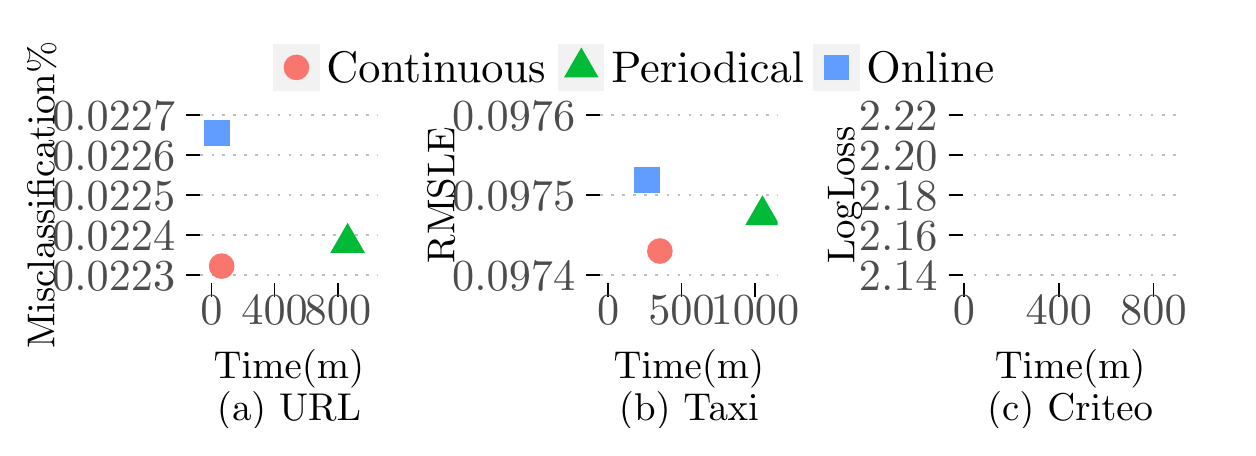
\begin{tikzpicture}[x=1pt,y=1pt]
\definecolor{fillColor}{RGB}{255,255,255}
\path[use as bounding box,fill=fillColor,fill opacity=0.00] (0,0) rectangle (433.62,144.54);
\begin{scope}
\path[clip] (  0.00,  0.00) rectangle (433.62,144.54);
\definecolor{fillColor}{RGB}{255,255,255}

\path[fill=fillColor] ( 78.42,115.81) rectangle (355.20,144.54);
\end{scope}
\begin{scope}
\path[clip] (  0.00,  0.00) rectangle (433.62,144.54);
\definecolor{drawColor}{RGB}{0,0,0}

\node[text=drawColor,anchor=base west,inner sep=0pt, outer sep=0pt, scale=  0.00] at ( 84.11,130.18) {Deployment};
\end{scope}
\begin{scope}
\path[clip] (  0.00,  0.00) rectangle (433.62,144.54);
\definecolor{drawColor}{RGB}{255,255,255}
\definecolor{fillColor}{gray}{0.95}

\path[draw=drawColor,line width= 0.6pt,line join=round,line cap=round,fill=fillColor] ( 88.44,121.50) rectangle (105.79,138.85);
\end{scope}
\begin{scope}
\path[clip] (  0.00,  0.00) rectangle (433.62,144.54);
\definecolor{fillColor}{RGB}{248,118,109}

\path[fill=fillColor] ( 97.12,130.18) circle (  4.64);
\end{scope}
\begin{scope}
\path[clip] (  0.00,  0.00) rectangle (433.62,144.54);
\definecolor{drawColor}{RGB}{255,255,255}
\definecolor{fillColor}{gray}{0.95}

\path[draw=drawColor,line width= 0.6pt,line join=round,line cap=round,fill=fillColor] (191.37,121.50) rectangle (208.72,138.85);
\end{scope}
\begin{scope}
\path[clip] (  0.00,  0.00) rectangle (433.62,144.54);
\definecolor{fillColor}{RGB}{0,186,56}

\path[fill=fillColor] (200.05,137.39) --
	(206.29,126.57) --
	(193.80,126.57) --
	cycle;
\end{scope}
\begin{scope}
\path[clip] (  0.00,  0.00) rectangle (433.62,144.54);
\definecolor{drawColor}{RGB}{255,255,255}
\definecolor{fillColor}{gray}{0.95}

\path[draw=drawColor,line width= 0.6pt,line join=round,line cap=round,fill=fillColor] (283.58,121.50) rectangle (300.92,138.85);
\end{scope}
\begin{scope}
\path[clip] (  0.00,  0.00) rectangle (433.62,144.54);
\definecolor{fillColor}{RGB}{97,156,255}

\path[fill=fillColor] (287.61,125.54) --
	(296.89,125.54) --
	(296.89,134.82) --
	(287.61,134.82) --
	cycle;
\end{scope}
\begin{scope}
\path[clip] (  0.00,  0.00) rectangle (433.62,144.54);
\definecolor{drawColor}{RGB}{0,0,0}

\node[text=drawColor,anchor=base west,inner sep=0pt, outer sep=0pt, scale=  1.60] at (107.96,124.67) {Continuous};
\end{scope}
\begin{scope}
\path[clip] (  0.00,  0.00) rectangle (433.62,144.54);
\definecolor{drawColor}{RGB}{0,0,0}

\node[text=drawColor,anchor=base west,inner sep=0pt, outer sep=0pt, scale=  1.60] at (210.89,124.67) {Periodical};
\end{scope}
\begin{scope}
\path[clip] (  0.00,  0.00) rectangle (433.62,144.54);
\definecolor{drawColor}{RGB}{0,0,0}

\node[text=drawColor,anchor=base west,inner sep=0pt, outer sep=0pt, scale=  1.60] at (303.09,124.67) {Online};
\end{scope}
\begin{scope}
\path[clip] (  0.00,  0.00) rectangle (144.54,115.81);
\definecolor{drawColor}{RGB}{255,255,255}
\definecolor{fillColor}{RGB}{255,255,255}

\path[draw=drawColor,line width= 0.6pt,line join=round,line cap=round,fill=fillColor] (  0.00,  0.00) rectangle (144.54,115.81);
\end{scope}
\begin{scope}
\path[clip] ( 62.30, 52.27) rectangle (126.47,115.81);
\definecolor{fillColor}{RGB}{255,255,255}

\path[fill=fillColor] ( 62.30, 52.27) rectangle (126.47,115.81);
\definecolor{drawColor}{RGB}{255,255,255}

\path[draw=drawColor,line width= 0.3pt,line join=round] ( 62.30, 62.38) --
	(126.47, 62.38);

\path[draw=drawColor,line width= 0.3pt,line join=round] ( 62.30, 76.82) --
	(126.47, 76.82);

\path[draw=drawColor,line width= 0.3pt,line join=round] ( 62.30, 91.26) --
	(126.47, 91.26);

\path[draw=drawColor,line width= 0.3pt,line join=round] ( 62.30,105.71) --
	(126.47,105.71);

\path[draw=drawColor,line width= 0.3pt,line join=round] ( 77.80, 52.27) --
	( 77.80,115.81);

\path[draw=drawColor,line width= 0.3pt,line join=round] (100.68, 52.27) --
	(100.68,115.81);

\path[draw=drawColor,line width= 0.3pt,line join=round] (123.56, 52.27) --
	(123.56,115.81);
\definecolor{drawColor}{RGB}{190,190,190}

\path[draw=drawColor,line width= 0.6pt,dash pattern=on 1pt off 3pt ,line join=round] ( 62.30, 55.16) --
	(126.47, 55.16);

\path[draw=drawColor,line width= 0.6pt,dash pattern=on 1pt off 3pt ,line join=round] ( 62.30, 69.60) --
	(126.47, 69.60);

\path[draw=drawColor,line width= 0.6pt,dash pattern=on 1pt off 3pt ,line join=round] ( 62.30, 84.04) --
	(126.47, 84.04);

\path[draw=drawColor,line width= 0.6pt,dash pattern=on 1pt off 3pt ,line join=round] ( 62.30, 98.49) --
	(126.47, 98.49);

\path[draw=drawColor,line width= 0.6pt,dash pattern=on 1pt off 3pt ,line join=round] ( 62.30,112.93) --
	(126.47,112.93);
\definecolor{drawColor}{RGB}{255,255,255}

\path[draw=drawColor,line width= 0.6pt,line join=round] ( 66.37, 52.27) --
	( 66.37,115.81);

\path[draw=drawColor,line width= 0.6pt,line join=round] ( 89.24, 52.27) --
	( 89.24,115.81);

\path[draw=drawColor,line width= 0.6pt,line join=round] (112.12, 52.27) --
	(112.12,115.81);
\definecolor{fillColor}{RGB}{97,156,255}

\path[fill=fillColor] ( 63.72,101.72) --
	( 73.00,101.72) --
	( 73.00,111.00) --
	( 63.72,111.00) --
	cycle;
\definecolor{fillColor}{RGB}{0,186,56}

\path[fill=fillColor] (115.61, 74.01) --
	(121.86, 63.18) --
	(109.36, 63.18) --
	cycle;
\definecolor{fillColor}{RGB}{248,118,109}

\path[fill=fillColor] ( 70.09, 58.38) circle (  4.64);
\end{scope}
\begin{scope}
\path[clip] (  0.00,  0.00) rectangle (433.62,144.54);
\definecolor{drawColor}{gray}{0.30}

\node[text=drawColor,anchor=base east,inner sep=0pt, outer sep=0pt, scale=  1.60] at ( 53.30, 49.65) {0.0223};

\node[text=drawColor,anchor=base east,inner sep=0pt, outer sep=0pt, scale=  1.60] at ( 53.30, 64.09) {0.0224};

\node[text=drawColor,anchor=base east,inner sep=0pt, outer sep=0pt, scale=  1.60] at ( 53.30, 78.53) {0.0225};

\node[text=drawColor,anchor=base east,inner sep=0pt, outer sep=0pt, scale=  1.60] at ( 53.30, 92.98) {0.0226};

\node[text=drawColor,anchor=base east,inner sep=0pt, outer sep=0pt, scale=  1.60] at ( 53.30,107.42) {0.0227};
\end{scope}
\begin{scope}
\path[clip] (  0.00,  0.00) rectangle (433.62,144.54);
\definecolor{drawColor}{RGB}{0,0,0}

\path[draw=drawColor,line width= 0.6pt,line join=round] ( 57.30, 55.16) --
	( 62.30, 55.16);

\path[draw=drawColor,line width= 0.6pt,line join=round] ( 57.30, 69.60) --
	( 62.30, 69.60);

\path[draw=drawColor,line width= 0.6pt,line join=round] ( 57.30, 84.04) --
	( 62.30, 84.04);

\path[draw=drawColor,line width= 0.6pt,line join=round] ( 57.30, 98.49) --
	( 62.30, 98.49);

\path[draw=drawColor,line width= 0.6pt,line join=round] ( 57.30,112.93) --
	( 62.30,112.93);
\end{scope}
\begin{scope}
\path[clip] (  0.00,  0.00) rectangle (433.62,144.54);
\definecolor{drawColor}{RGB}{0,0,0}

\path[draw=drawColor,line width= 0.6pt,line join=round] ( 66.37, 47.27) --
	( 66.37, 52.27);

\path[draw=drawColor,line width= 0.6pt,line join=round] ( 89.24, 47.27) --
	( 89.24, 52.27);

\path[draw=drawColor,line width= 0.6pt,line join=round] (112.12, 47.27) --
	(112.12, 52.27);
\end{scope}
\begin{scope}
\path[clip] (  0.00,  0.00) rectangle (433.62,144.54);
\definecolor{drawColor}{gray}{0.30}

\node[text=drawColor,anchor=base,inner sep=0pt, outer sep=0pt, scale=  1.60] at ( 66.37, 37.26) {0};

\node[text=drawColor,anchor=base,inner sep=0pt, outer sep=0pt, scale=  1.60] at ( 89.24, 37.26) {400};

\node[text=drawColor,anchor=base,inner sep=0pt, outer sep=0pt, scale=  1.60] at (112.12, 37.26) {800};
\end{scope}
\begin{scope}
\path[clip] (  0.00,  0.00) rectangle (433.62,144.54);
\definecolor{drawColor}{RGB}{0,0,0}

\node[text=drawColor,anchor=base,inner sep=0pt, outer sep=0pt, scale=  1.40] at ( 94.39, 17.61) {Time(m)};

\node[text=drawColor,anchor=base,inner sep=0pt, outer sep=0pt, scale=  1.40] at ( 94.39,  2.49) {(a) URL};
\end{scope}
\begin{scope}
\path[clip] (  0.00,  0.00) rectangle (433.62,144.54);
\definecolor{drawColor}{RGB}{0,0,0}

\node[text=drawColor,rotate= 90.00,anchor=base,inner sep=0pt, outer sep=0pt, scale=  1.40] at (  9.64, 84.04) {Misclassification\%};
\end{scope}
\begin{scope}
\path[clip] (144.54,  0.00) rectangle (289.08,115.81);
\definecolor{drawColor}{RGB}{255,255,255}
\definecolor{fillColor}{RGB}{255,255,255}

\path[draw=drawColor,line width= 0.6pt,line join=round,line cap=round,fill=fillColor] (144.54,  0.00) rectangle (289.08,115.81);
\end{scope}
\begin{scope}
\path[clip] (206.84, 52.27) rectangle (271.01,115.81);
\definecolor{fillColor}{RGB}{255,255,255}

\path[fill=fillColor] (206.84, 52.27) rectangle (271.01,115.81);
\definecolor{drawColor}{RGB}{255,255,255}

\path[draw=drawColor,line width= 0.3pt,line join=round] (206.84, 69.60) --
	(271.01, 69.60);

\path[draw=drawColor,line width= 0.3pt,line join=round] (206.84, 98.49) --
	(271.01, 98.49);

\path[draw=drawColor,line width= 0.3pt,line join=round] (223.02, 52.27) --
	(223.02,115.81);

\path[draw=drawColor,line width= 0.3pt,line join=round] (249.53, 52.27) --
	(249.53,115.81);
\definecolor{drawColor}{RGB}{190,190,190}

\path[draw=drawColor,line width= 0.6pt,dash pattern=on 1pt off 3pt ,line join=round] (206.84, 55.16) --
	(271.01, 55.16);

\path[draw=drawColor,line width= 0.6pt,dash pattern=on 1pt off 3pt ,line join=round] (206.84, 84.04) --
	(271.01, 84.04);

\path[draw=drawColor,line width= 0.6pt,dash pattern=on 1pt off 3pt ,line join=round] (206.84,112.93) --
	(271.01,112.93);
\definecolor{drawColor}{RGB}{255,255,255}

\path[draw=drawColor,line width= 0.6pt,line join=round] (209.76, 52.27) --
	(209.76,115.81);

\path[draw=drawColor,line width= 0.6pt,line join=round] (236.28, 52.27) --
	(236.28,115.81);

\path[draw=drawColor,line width= 0.6pt,line join=round] (262.79, 52.27) --
	(262.79,115.81);
\definecolor{fillColor}{RGB}{97,156,255}

\path[fill=fillColor] (219.04, 84.86) --
	(228.32, 84.86) --
	(228.32, 94.14) --
	(219.04, 94.14) --
	cycle;
\definecolor{fillColor}{RGB}{0,186,56}

\path[fill=fillColor] (265.52, 83.97) --
	(271.76, 73.15) --
	(259.27, 73.15) --
	cycle;
\definecolor{fillColor}{RGB}{248,118,109}

\path[fill=fillColor] (228.43, 63.83) circle (  4.64);
\end{scope}
\begin{scope}
\path[clip] (  0.00,  0.00) rectangle (433.62,144.54);
\definecolor{drawColor}{gray}{0.30}

\node[text=drawColor,anchor=base east,inner sep=0pt, outer sep=0pt, scale=  1.60] at (197.84, 49.65) {0.0974};

\node[text=drawColor,anchor=base east,inner sep=0pt, outer sep=0pt, scale=  1.60] at (197.84, 78.53) {0.0975};

\node[text=drawColor,anchor=base east,inner sep=0pt, outer sep=0pt, scale=  1.60] at (197.84,107.42) {0.0976};
\end{scope}
\begin{scope}
\path[clip] (  0.00,  0.00) rectangle (433.62,144.54);
\definecolor{drawColor}{RGB}{0,0,0}

\path[draw=drawColor,line width= 0.6pt,line join=round] (201.84, 55.16) --
	(206.84, 55.16);

\path[draw=drawColor,line width= 0.6pt,line join=round] (201.84, 84.04) --
	(206.84, 84.04);

\path[draw=drawColor,line width= 0.6pt,line join=round] (201.84,112.93) --
	(206.84,112.93);
\end{scope}
\begin{scope}
\path[clip] (  0.00,  0.00) rectangle (433.62,144.54);
\definecolor{drawColor}{RGB}{0,0,0}

\path[draw=drawColor,line width= 0.6pt,line join=round] (209.76, 47.27) --
	(209.76, 52.27);

\path[draw=drawColor,line width= 0.6pt,line join=round] (236.28, 47.27) --
	(236.28, 52.27);

\path[draw=drawColor,line width= 0.6pt,line join=round] (262.79, 47.27) --
	(262.79, 52.27);
\end{scope}
\begin{scope}
\path[clip] (  0.00,  0.00) rectangle (433.62,144.54);
\definecolor{drawColor}{gray}{0.30}

\node[text=drawColor,anchor=base,inner sep=0pt, outer sep=0pt, scale=  1.60] at (209.76, 37.26) {0};

\node[text=drawColor,anchor=base,inner sep=0pt, outer sep=0pt, scale=  1.60] at (236.28, 37.26) {500};

\node[text=drawColor,anchor=base,inner sep=0pt, outer sep=0pt, scale=  1.60] at (262.79, 37.26) {1000};
\end{scope}
\begin{scope}
\path[clip] (  0.00,  0.00) rectangle (433.62,144.54);
\definecolor{drawColor}{RGB}{0,0,0}

\node[text=drawColor,anchor=base,inner sep=0pt, outer sep=0pt, scale=  1.40] at (238.93, 17.61) {Time(m)};

\node[text=drawColor,anchor=base,inner sep=0pt, outer sep=0pt, scale=  1.40] at (238.93,  2.49) {(b) Taxi};
\end{scope}
\begin{scope}
\path[clip] (  0.00,  0.00) rectangle (433.62,144.54);
\definecolor{drawColor}{RGB}{0,0,0}

\node[text=drawColor,rotate= 90.00,anchor=base,inner sep=0pt, outer sep=0pt, scale=  1.40] at (154.18, 84.04) {RMSLE};
\end{scope}
\begin{scope}
\path[clip] (289.08,  0.00) rectangle (433.62,115.81);
\definecolor{drawColor}{RGB}{255,255,255}
\definecolor{fillColor}{RGB}{255,255,255}

\path[draw=drawColor,line width= 0.6pt,line join=round,line cap=round,fill=fillColor] (289.08,  0.00) rectangle (433.62,115.81);
\end{scope}
\begin{scope}
\path[clip] (337.81, 52.27) rectangle (415.55,115.81);
\definecolor{fillColor}{RGB}{255,255,255}

\path[fill=fillColor] (337.81, 52.27) rectangle (415.55,115.81);
\definecolor{drawColor}{RGB}{255,255,255}

\path[draw=drawColor,line width= 0.3pt,line join=round] (337.81, 62.38) --
	(415.55, 62.38);

\path[draw=drawColor,line width= 0.3pt,line join=round] (337.81, 76.82) --
	(415.55, 76.82);

\path[draw=drawColor,line width= 0.3pt,line join=round] (337.81, 91.26) --
	(415.55, 91.26);

\path[draw=drawColor,line width= 0.3pt,line join=round] (337.81,105.71) --
	(415.55,105.71);

\path[draw=drawColor,line width= 0.3pt,line join=round] (355.47, 52.27) --
	(355.47,115.81);

\path[draw=drawColor,line width= 0.3pt,line join=round] (389.69, 52.27) --
	(389.69,115.81);
\definecolor{drawColor}{RGB}{190,190,190}

\path[draw=drawColor,line width= 0.6pt,dash pattern=on 1pt off 3pt ,line join=round] (337.81, 55.16) --
	(415.55, 55.16);

\path[draw=drawColor,line width= 0.6pt,dash pattern=on 1pt off 3pt ,line join=round] (337.81, 69.60) --
	(415.55, 69.60);

\path[draw=drawColor,line width= 0.6pt,dash pattern=on 1pt off 3pt ,line join=round] (337.81, 84.04) --
	(415.55, 84.04);

\path[draw=drawColor,line width= 0.6pt,dash pattern=on 1pt off 3pt ,line join=round] (337.81, 98.49) --
	(415.55, 98.49);

\path[draw=drawColor,line width= 0.6pt,dash pattern=on 1pt off 3pt ,line join=round] (337.81,112.93) --
	(415.55,112.93);
\definecolor{drawColor}{RGB}{255,255,255}

\path[draw=drawColor,line width= 0.6pt,line join=round] (338.36, 52.27) --
	(338.36,115.81);

\path[draw=drawColor,line width= 0.6pt,line join=round] (372.58, 52.27) --
	(372.58,115.81);

\path[draw=drawColor,line width= 0.6pt,line join=round] (406.80, 52.27) --
	(406.80,115.81);
\end{scope}
\begin{scope}
\path[clip] (  0.00,  0.00) rectangle (433.62,144.54);
\definecolor{drawColor}{gray}{0.30}

\node[text=drawColor,anchor=base east,inner sep=0pt, outer sep=0pt, scale=  1.60] at (328.81, 49.65) {2.14};

\node[text=drawColor,anchor=base east,inner sep=0pt, outer sep=0pt, scale=  1.60] at (328.81, 64.09) {2.16};

\node[text=drawColor,anchor=base east,inner sep=0pt, outer sep=0pt, scale=  1.60] at (328.81, 78.53) {2.18};

\node[text=drawColor,anchor=base east,inner sep=0pt, outer sep=0pt, scale=  1.60] at (328.81, 92.98) {2.20};

\node[text=drawColor,anchor=base east,inner sep=0pt, outer sep=0pt, scale=  1.60] at (328.81,107.42) {2.22};
\end{scope}
\begin{scope}
\path[clip] (  0.00,  0.00) rectangle (433.62,144.54);
\definecolor{drawColor}{RGB}{0,0,0}

\path[draw=drawColor,line width= 0.6pt,line join=round] (332.81, 55.16) --
	(337.81, 55.16);

\path[draw=drawColor,line width= 0.6pt,line join=round] (332.81, 69.60) --
	(337.81, 69.60);

\path[draw=drawColor,line width= 0.6pt,line join=round] (332.81, 84.04) --
	(337.81, 84.04);

\path[draw=drawColor,line width= 0.6pt,line join=round] (332.81, 98.49) --
	(337.81, 98.49);

\path[draw=drawColor,line width= 0.6pt,line join=round] (332.81,112.93) --
	(337.81,112.93);
\end{scope}
\begin{scope}
\path[clip] (  0.00,  0.00) rectangle (433.62,144.54);
\definecolor{drawColor}{RGB}{0,0,0}

\path[draw=drawColor,line width= 0.6pt,line join=round] (338.36, 47.27) --
	(338.36, 52.27);

\path[draw=drawColor,line width= 0.6pt,line join=round] (372.58, 47.27) --
	(372.58, 52.27);

\path[draw=drawColor,line width= 0.6pt,line join=round] (406.80, 47.27) --
	(406.80, 52.27);
\end{scope}
\begin{scope}
\path[clip] (  0.00,  0.00) rectangle (433.62,144.54);
\definecolor{drawColor}{gray}{0.30}

\node[text=drawColor,anchor=base,inner sep=0pt, outer sep=0pt, scale=  1.60] at (338.36, 37.26) {0};

\node[text=drawColor,anchor=base,inner sep=0pt, outer sep=0pt, scale=  1.60] at (372.58, 37.26) {400};

\node[text=drawColor,anchor=base,inner sep=0pt, outer sep=0pt, scale=  1.60] at (406.80, 37.26) {800};
\end{scope}
\begin{scope}
\path[clip] (  0.00,  0.00) rectangle (433.62,144.54);
\definecolor{drawColor}{RGB}{0,0,0}

\node[text=drawColor,anchor=base,inner sep=0pt, outer sep=0pt, scale=  1.40] at (376.68, 17.61) {Time(m)};

\node[text=drawColor,anchor=base,inner sep=0pt, outer sep=0pt, scale=  1.40] at (376.68,  2.49) {(c) Criteo};
\end{scope}
\begin{scope}
\path[clip] (  0.00,  0.00) rectangle (433.62,144.54);
\definecolor{drawColor}{RGB}{0,0,0}

\node[text=drawColor,rotate= 90.00,anchor=base,inner sep=0pt, outer sep=0pt, scale=  1.40] at (298.72, 84.04) {LogLoss};
\end{scope}
\end{tikzpicture}
